\clearpage
\section{本人素材与情绪立绘生成流程}
\label{sec:design-generation}
用户可以在形象设置里管理头像、背景和个人立绘。头像用来辨认用户，背景用于个人页面，立绘用于真人聊天中的本人展示。生成情绪图要先有默认立绘，以保持不同表情下的人物外观一致。

用户选择情绪，并授权将默认立绘发送给 AI 服务后，后台开始生成。相同账号用同一请求编号重试同一情绪时，服务端复用原任务。等待期间可以继续聊天，也可以在设置页查看进度。一个账号同一时间只能有一个生成中或待确认的任务，待确认的结果要先保存或放弃，之后才能发起下一次生成。滚动 24 小时内每个账号最多创建 12 个生成任务，服务端同时运行的生成任务最多 2 个。

\begin{figure}[H]
\centering
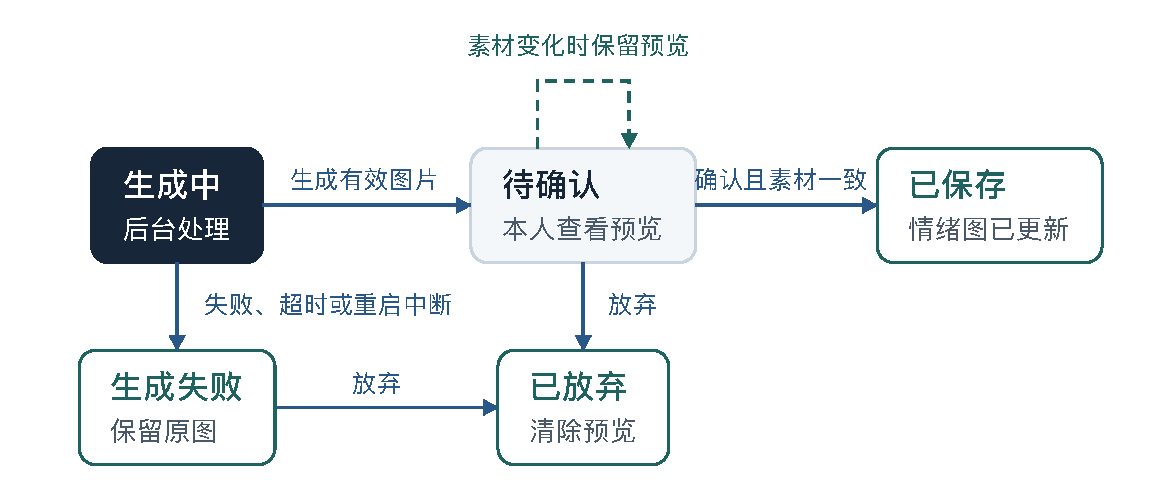
\includegraphics[width=\linewidth]{assets/design/portrait-generation.pdf}
\caption{情绪立绘从生成到确认的状态流转}\label{fig:design-generation}
\end{figure}

图片通过检查后，只有本人能看到预览。以开心立绘为例，用户可以先检查表情和人物形象是否合适，确认后，图片保存为开心状态下的立绘，供真人聊天读取。用户也可以放弃预览。生成失败时保留现有立绘，并提示重试。

